\documentclass[12pt]{article}
\usepackage{geometry}
\usepackage{graphicx}
\usepackage{pdfpages}
\usepackage[utf8]{inputenc}
\geometry{lmargin=2cm,rmargin=1cm,tmargin=2cm,bmargin=2cm}
\renewcommand{\baselinestretch}{1.5} 

\begin{document}
\pagenumbering{gobble}

\begin{center}
	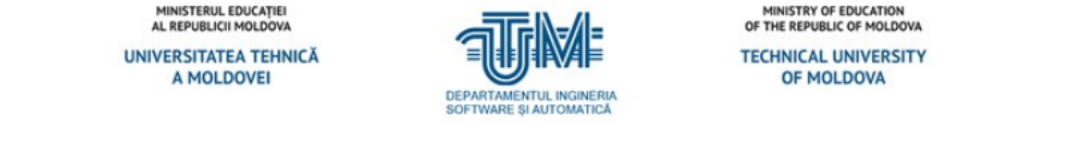
\includegraphics[scale=0.5]{img_title_amsi} 
\end{center} 
\ \\
\begin{flushright}
	\textbf{{\fontsize{14}{10}\selectfont Discipline: Network programming}}
\end{flushright}
\ \\
\ \\
\ \\

\begin{center}
	\textbf{{\fontsize{15}{10}\selectfont Laboratory Work nr.2 \\
	\underline{Topic:} Metrics Aggregator.}}
\end{center}
\ \\
\ \\
\ \\
\ \\
\ \\
\begin{flushright}
	{\fontsize{12}{10}\selectfont 
		\textbf{Done by student:}  \rule{2cm}{0.4pt}(Untilov Andrei, gr.FAF-151) \\
		\ \\
		\ \\
		\textbf{Verified by:}      \rule{2cm}{0.4pt}(Gavrișco Alexandru)
		
		}
\end{flushright}
\vfill

\begin{center}
	\textbf{Chisinau 2018}
\end{center}

\newpage
\pagenumbering{arabic}
\setcounter{page}{2}
	\tableofcontents
	\newpage
	
	\section{Topic}
	Metrics Aggregator.
	\section{Tasks}
	\begin{enumerate}
		\item Request your secret key at https://desolate-ravine-43301.herokuapp.com/, in response you'll receive a list of URLs (for each device);
		\item Using your secret key, request data from all devices concurrently;
		\item If you get an error related to your access key, go back to step 1 and retry;
		\item Parse data from all devices;
		\item Aggregate all responses ordering by sensor type.
	\end{enumerate}
	

	\newpage
	\section{Task Implementation}
	
	In order to perform this laboratory work, was developed an Android application.
	
	\subsection{Request your secret key}
	The request of secret key was performed in LinkConnector.class , extending AsyncTask.class . Basically was created a HttpClient which exectued an HttpPost request, providing the URL. From response was extracted the secret key as follows "response.getFirstHeader("Session").getValue()".
	Also, has been retrived the list of links from the provided json, and converted to Link objects.
	
	
	
	
	
	\subsection{Using your secret key, request data from all devices concurrently}
	In a separated thread, for every Link from linksList was exectued a GET request and retrieved devices data.The code is provided by method "performTask" of DeviceConnector.class.
	
	\subsection{Parse data from all devices}
	Every response is handled according to the detected type of data( CSV, XML or JSON),and converted to Devices objects.The code is provided by methods "parseCSV" , "parseXML" and "parseJSON" of DeviceConnector.class.
	
	\subsection{Aggregate all responses ordering by sensor type.}
	After the conversion to Java objects, the data is aggregated. The code is provided by method "aggregateData" of DeviceConnector.class.
	
	*The source code
	
	
	
	
	
	
\end{document}
